\documentclass{article}
\usepackage[utf8]{inputenc}
\usepackage{polski}
\usepackage{booktabs}
\usepackage[margin=1in]{geometry}
\usepackage{graphicx}
\usepackage{float}
\usepackage{outlines}


\begin{document}
\begin{titlepage}

\newcommand{\HRule}{\rule{\linewidth}{0.5mm}}
\center
 
\textsc{\LARGE Politechnika Wrocławska}\\[1.5cm] 
\textsc{\Large bazy danych}\\[1cm] %TU

\HRule \\[0.5cm]
{ \Large \bfseries Mobilne stacje pogodowe}\\[0.5cm] %TU
\HRule \\[1cm]
 Grupa V\\
 termin zajęć: piątek 11:15\\[1cm]
\begin{minipage}[t]{0.4\textwidth}
\begin{flushleft} \large
\emph{Autorzy:}\\
 Michał Kuczaj \space 235920 \\
 Michał Cichocki \space 235986\\
 Kacper Maj \space 235348
\end{flushleft}
\end{minipage}
~
\begin{minipage}[t]{0.4\textwidth}
\begin{flushright} \large
\emph{Prowadzący:} \\
dr inż. Roman Ptak %TU
\end{flushright}
\end{minipage}\\[4cm]

\vfill
{\large \today }\\[2cm] %TU %TU


\end{titlepage}


\tableofcontents
\newpage%
% ====================================

\section{Wstęp}
\subsection{Cel projektu}
Głównym celem projektu jest zapewnienie obsługi dla  danych dostarczanych przez mobilne stacje pogodowe, a następnie udostępnianie ich dla dla użytkowników systemu przez serwis internetowy.
\subsection{Zakres projektu}
W zakres projektu wchodzi stworzenie bazy danych na serwerze, a następnie ich obsługa i dostarczenie do użytkownika w przystępnej formie.
% Dane z mobilnych stacji pogodowych zbierane będą na serwerze a następnie obsługiwane i wyświetlane w serwisie internetowym.

\section{Analiza wymagań}
    % Wybór i opracowanie wstępnych założeń dotyczących wybranych tematów projektów.
\subsection{Opis działania i schemat logiczny systemu}
    % Opis słowny systemu i jego otoczenia. 
    Projekt składać się będzie z sieci niedużych, bezprzewodowych, przenośnych stacji pogodowych działających na zasilaniu bateryjnym. Stacje będą ulokowane w różnych miejscach miasta wybranych przez użytkownika.
    Dane ze stacji zbierane będą na serwerze a następnie obsługiwane i wyświetlane w serwisie internetowym.

    Zbierane dane to: ciśnienie, temperatura i wilgotność w wybranych przez użytkowania interwałach czasu. Dodatkowo każda stacja w bazie danych musi mieć zarezerwowane miejsce na dane takie jak np.: lokalizacja, nazwa nadana przez użytkownika, stan baterii itd.
    
    Użytkownik systemu będzie mógł gromadzić dane prywatnie, lub udostępniać je publicznie.
    Każda stacja pogodowa będzie miała wygenerowany i przypisany swój unikalny numer ID.
    
    \begin{figure}[h]
        \centering
        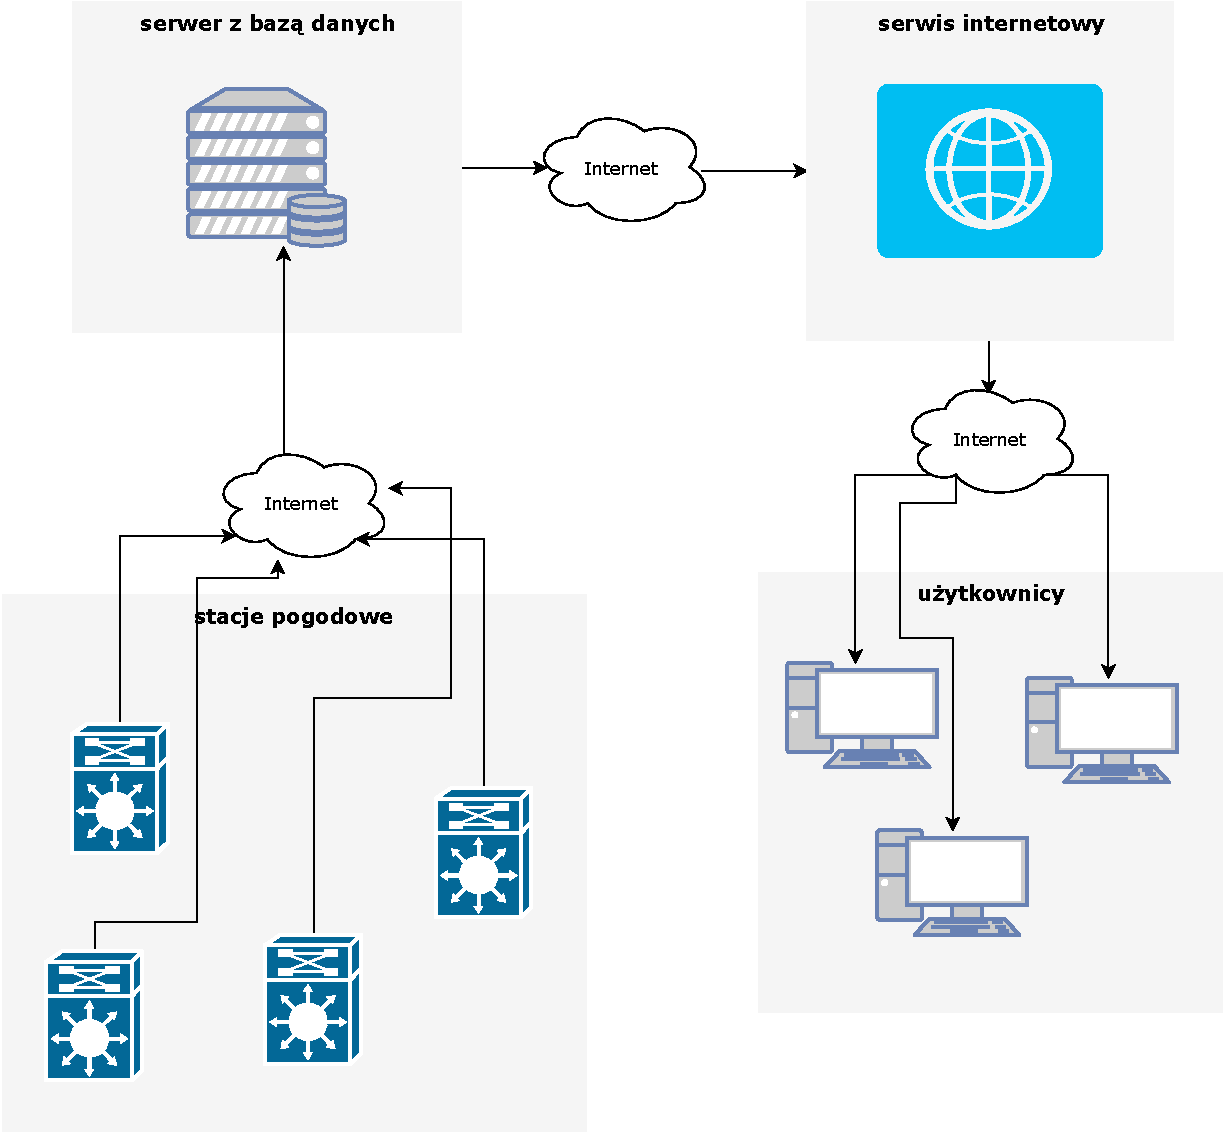
\includegraphics[width=0.5\linewidth]{ogolne.pdf}
        \caption{Ogólny schemat logiczny}
        \label{fig:schemat}
    \end{figure}
\newpage
\subsection{Wymagania funkcjonalne}
    % Opis funkcjonalności (możliwości) systemu, wyszczególnienie jego funkcji.
    
Cały system będzie opierał się na 4 rodzajach użytkowników. Pierwszy z nich to \textbf{administrator} całego systemu mający uprawnienia do zarządzania nim w każdym stopniu i na każdym poziomie. Kolejny rodzaj użytkownika to \textbf{użytkownik prywatny} mający dostęp do swojej stacji pogodowej, dzięki czemu może zarządzać, które dane mają być udostępniane do ogólnodostępnej bazy danych. Kolejny to \textbf{użytkownik publiczny}, który ma dostęp do wszystkich danych (udostępnionych przez użytkowników prywatnych), ale nie ma możliwości w żaden sposób ingerować w system. Ostatnim rodzajem użytkownika to sama \textbf{stacja pogodowa} (jako urządzenie).
    \begin{outline}
        \1 akwizycja danych 
            \2 zbierane dane: data, czas, ciśnienie, temperatura, wilgotność
            \2 podstawowe operacje CRUD
            \2 wyszukiwanie danych
            \2 sporządzenie statystyk
        \1 serwis internetowy
            \2 możliwość założenia konta użytkownika
            \2 możliwość upublicznienia zbieranych danych
    \end{outline}
\subsection{Wymagania niefunkcjonalne}
\subsubsection{Wykorzystywane technologie i narzędzia}
    Do stworzenia bazy wykorzystany zostanie \textbf{MySQL} czyli narzędzie dostarczone przez Oracle. MySQL został wybrany, ponieważ jest najbardziej popularnym systemem zarządzania bazą danych. Posiada doskonałą dokumentacje, możemy znaleźć bardzo dużo informacji na jego temat w literaturze. Na dzisiejszym rynku pracy wyróżnia się głownie MySQL jako niezbędny element, który programista musi znać.\\
    Język w jakim będziemy pracować to \textbf{Python}. Jest on na tyle uniwersalny i prosty, że możemy się go nauczyć przy tym projekcie, a następnie stosować do własnych potrzeb. Dodatkowo porównując dokumentację dostarczoną przez Oracle, tworzenie bazy danych w tym języku jest dużo prostsze i nie wymaga skupiania swojej uwagi na mniej znaczących aspektach jak np. poprawny wskaźnik do danych lub iterator wychodzący poza dozwolony obszar pamięci.
    \subsubsection{Wymagania dotyczące rozmiaru bazy danych}
    Około 100 użytkowników, każdy średnio po 5 stacji pogodowych.\\
    Stacje będą pracowały w zdefiniowanych przez użytkownika interwałach. W przypadku kiedy interwał jest najniższy dane przesyłane są co 10 min.\\
    Przy założeniu że baza będzie obciążona maksymalnie będzie otrzymywała dane co 10 min z około 500 stacji pogodowych.\\
    Otrzymywane dane to: temperatura, wilgotność, ciśnienie (float). Do danych będzie dodawana godzina i data przez bazę.\\
    Szacunkowo kiedy dane będą przechowywane przez rok? \\
    3x4(float-temp,ciśnienie,wilgotność)+5(godzina)*144(ilość wpisów w ciągu doby)*500(stacji pogodowych) / 1024(na kB)/1024(na Mb) = 4.11 MB dziennie.\\
    4.11*365 = 1.5 Gb na rok.\\
    Przy założeniu że będzie maksymalne obciążenie.\\
    Do tego jakieś dane z danymi stacji, użytkowników itd.
    Mozna ograniczyć baze do nadpisywania po roku wtedy nie przekroczy 2 Gb.
    
\subsubsection{Wymagania dotyczące bezpieczeństwa systemu}
    Standardowy system logowania. Hasła przechowywane w formie zaszyfrowanej.
\subsection{Przyjęte założenia projektowe}



% ====================================
% \newpage
% \addcontentsline{toc}{section}{Literatura}
% \bibliographystyle{plain}
% \nocite{*}
% \bibliography{./bibliografia}
% \addcontentsline{toc}{section}{Spis rysunków}
% \listoffigures
% \addcontentsline{toc}{section}{Spis tabel}
% \listoftables

\end{document}